%
\hsection{pip and Virtual Environments}%
\label{sec:pipAndVenv}%
%
The go-to tool for installing \python\ \pglspl{package} is \pip~\cite{PSF:P3D:IPM,PD2024PD}.%
%
\usefulTool{pip}{%
\pip\ is a software that can be used to install \pglspl{package} under \python. %
\begin{itemize}%
\item With the command \bashil{pip install thePackage}, the \pgls{package}~\bashil{thePackage} is installed.%
\item With the command \bashil{pip install "thePackage==version"}, the version~\bashil{version} of the \pgls{package}~\bashil{thePackage} is installed.%
\item With the command \bashil{pip install -r requirements.txt}, the \pglspl{package} listed in the requirements file \textil{requirements.txt} are installed. %
A requirements file allows to put multiple package/version dependencies that would otherwise command line arguments of \pip\ into a single file~\cite{PD2024PD:RFF}.%
\end{itemize}%
%
\pip\ should always be used in a \pgls{virtualEnvironment}, see~\cref{bp:venvInstall,bp:pipVenv}.%
}%
%
The standard way to install \pglspl{package} for use with \python\ is in a so-called \pgls{virtualEnvironment}.
A \pgls{virtualEnvironment} is a directory with an isolated \python\ installation and \pgls{package} directory~\cite{PSF:P3D:TPT:VEAP,PEP405}.
Multiple separate \pglspl{virtualEnvironment} can exist on a computer, all with their own set of installed \pglspl{package}.
This allows you to have different \python\ setups for different applications by installing them into different \pglspl{virtualEnvironment}.
\Pglspl{virtualEnvironment} are particularly useful if different applications need different versions of the same \pglspl{package}.
This way, version clashes are avoided.
They also give you better understanding about the actual dependencies of your applications:
Installing the \pglspl{package} directly needed by an application into a new \pgls{virtualEnvironment} will also install their dependencies and the dependencies of their dependencies, and so on.%
%
\bestPractice{venvInstall}{%
\Pglspl{package} should \emph{always} be installed in \pglspl{virtualEnvironment} and never system-wide (maybe with the exception of \pip\ and \venv).%
}%
%
\bestPractice{pipVenv}{\sloppy%
The command \bashil{pip install} should always be used with the option \bashil{--require-virtualenv}, e.g., \bashil{pip install --require-virtualenv thePackage}. %
This enforces that \pip\ is really executed in a \pgls{virtualEnvironment} and will cause an error otherwise.%
}%
%
\usefulTool{venv}{The module \venv\ is used for creating and managing \pglspl{virtualEnvironment} under \python.}%
%
\gitLoadPython{packages:numpy_user}{}{packages/numpy_user.py}{}%
\listingPython{packages:numpy_user}{%
A small \python\ script using the \numpy\ library.}%
%
For demonstration purposes, let us assume that we have written a program using the \pgls{package} \numpy~\cite{HMvdWGVCWTBSKPHvKBHFdRWPGMSRWAGO2020APWN,DBvR2024ITN,J2018NPSCADSAWNSAM}.
The small program in \cref{lst:packages:numpy_user} only creates and prints a \numpy\ array, but for this, obviously, \numpy\ is needed.
\numpy\ is not available in fresh \python\ installations and needs to be installed so that we can run our program.
This will be the example that we will use to demonstrate the use of \pglspl{virtualEnvironment} in the following sections.

As prerequisites to install \pglspl{package} in \pglspl{virtualEnvironment}, we need to make sure that both \pip\ and \venv\ are installed on our system.
The procedures for both differ under \linux\ and \microsoftWindows.
Using \pip\ and \venv\ is often done in the \pgls{terminal}, i.e., by typing commands or executing shell scripts.
This, naturally, too works differently under \linux\ and \microsoftWindows.
We therefore will briefly explore how to achieve these things under both operating systems.%
%
\FloatBarrier%
\hsection{pip and Virtual Environments in Ubuntu Linux}%
%
\begin{figure}%
\centering%
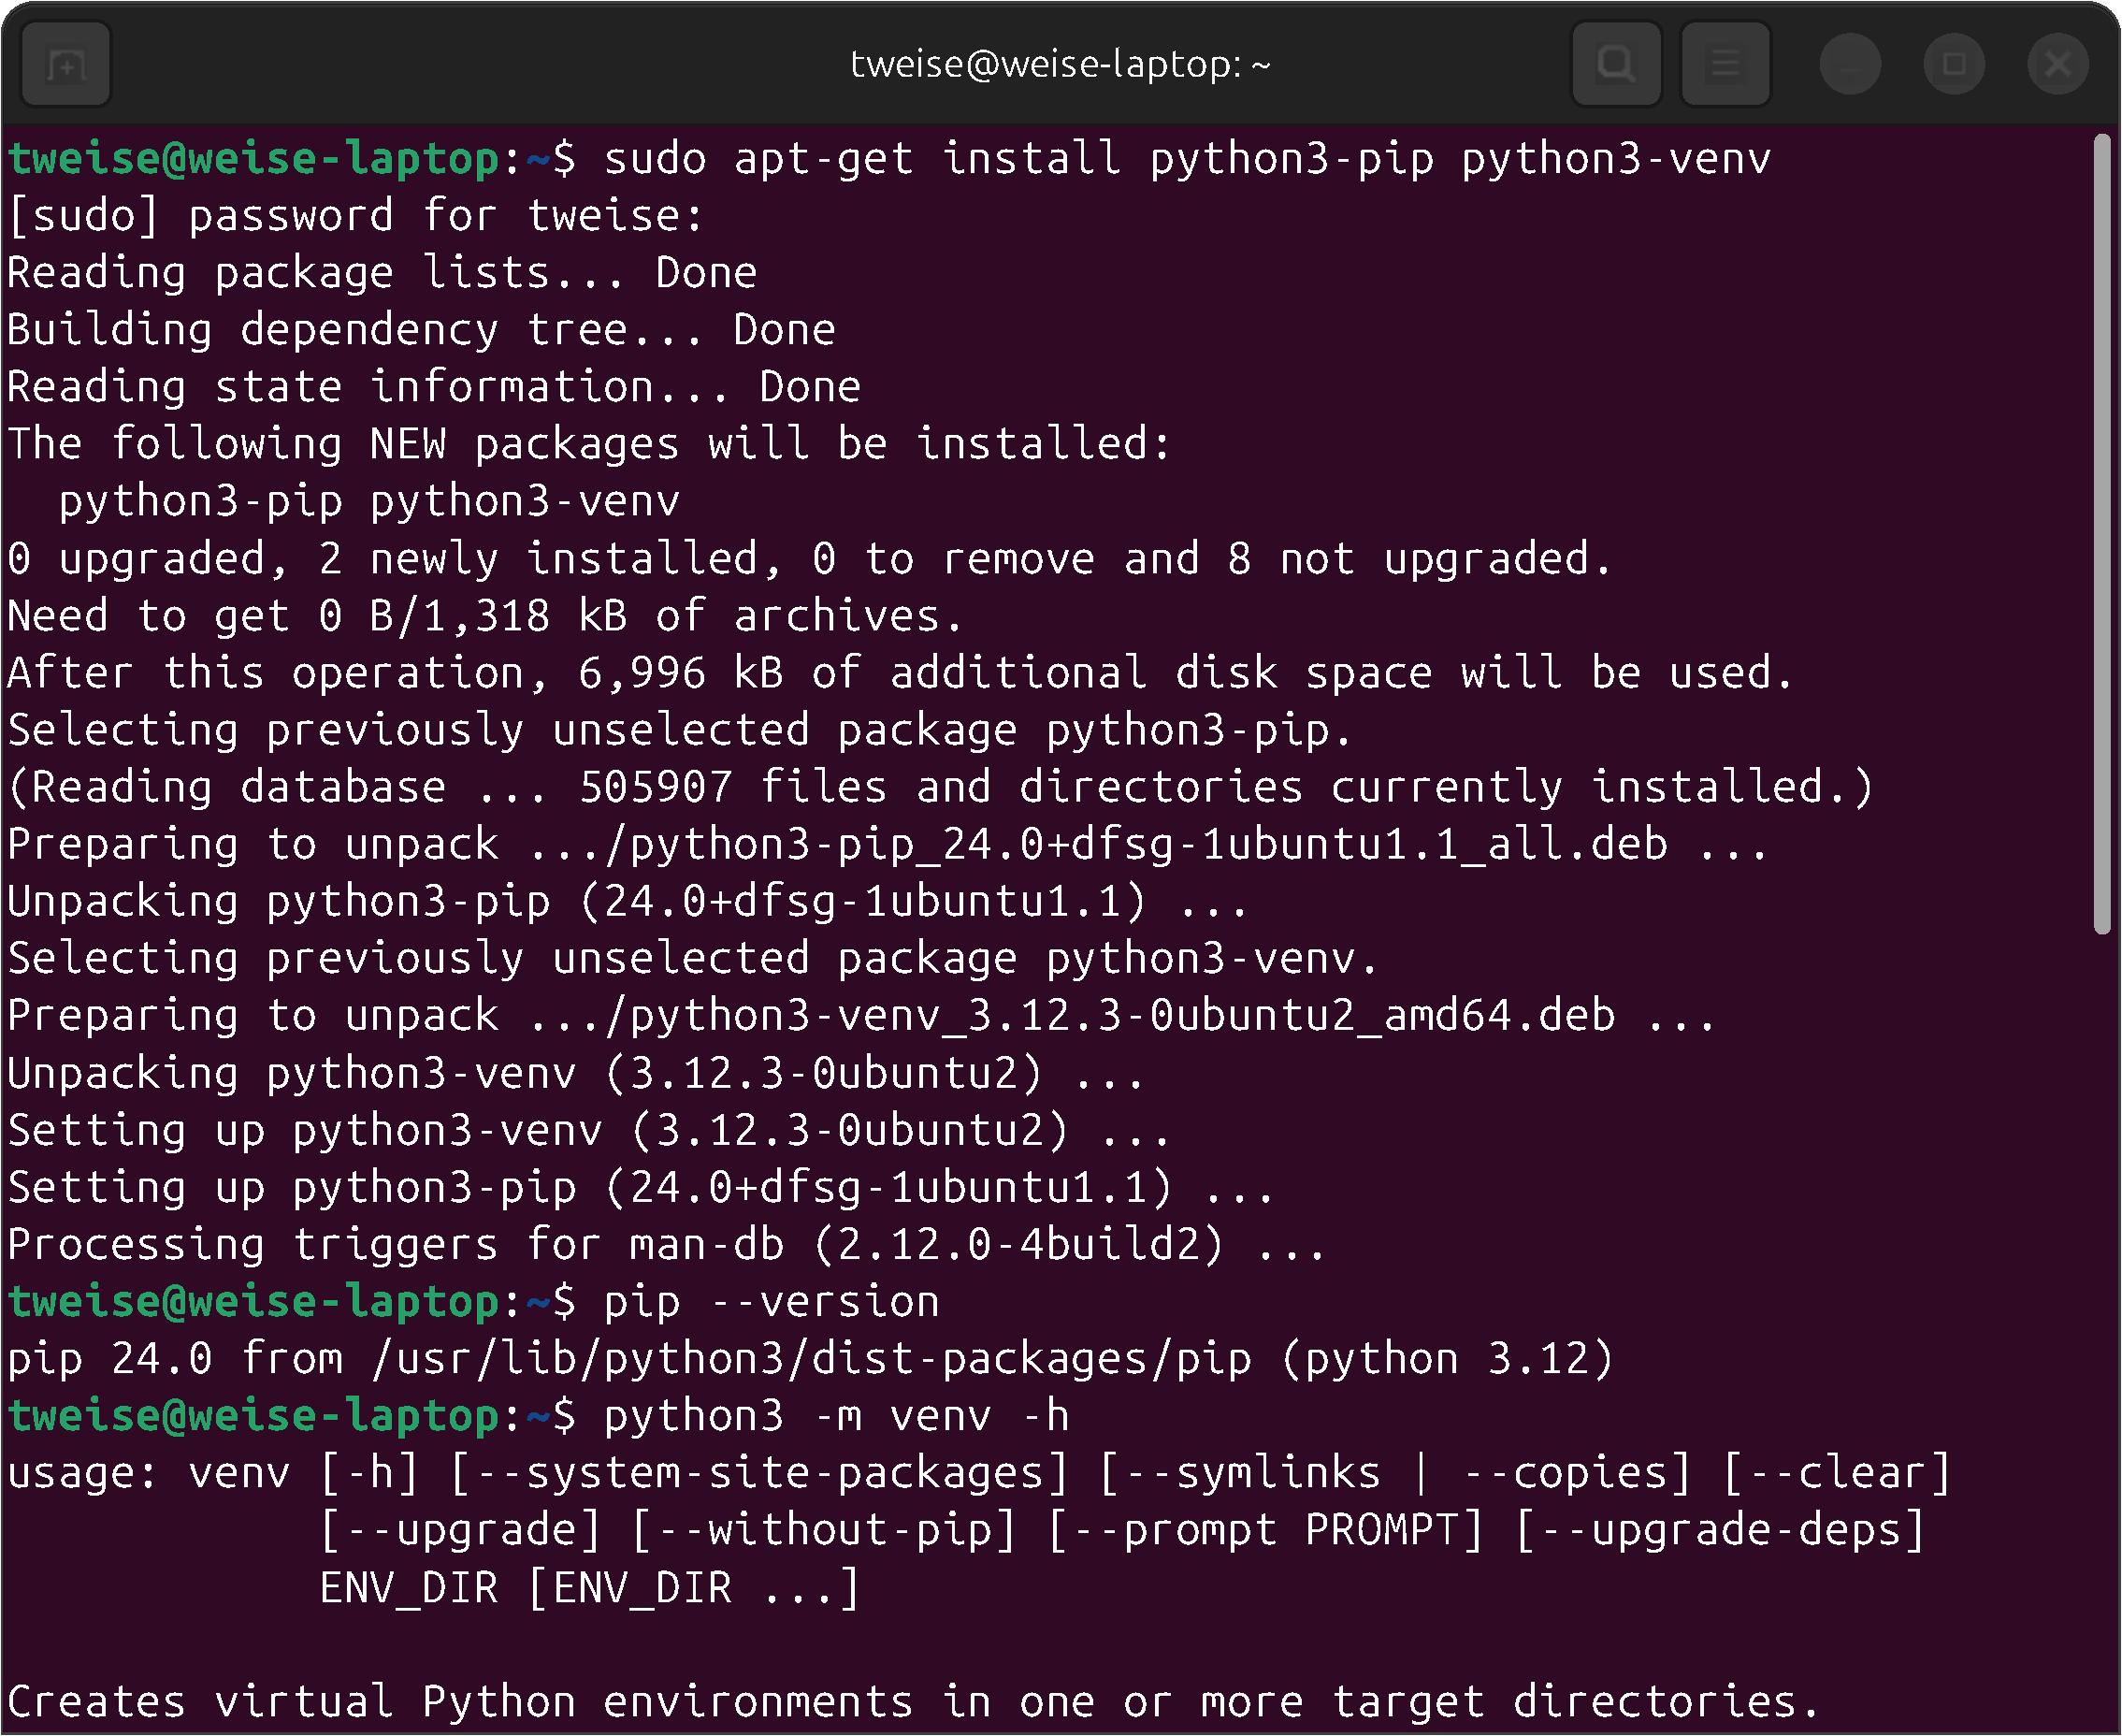
\includegraphics[width=0.7\linewidth]{\currentDir/installPipVenvUbuntu}%
\caption{Installing \pip\ and venv under \ubuntu\ \linux: \pip~is usually already installed, \venv\ maybe or maybe not. %
We need to use the \bashil{apt-get} route to make sure that both \bashil{python3-pip} and \bashil{python3-venv} are installed.}%
\label{fig:installPipVenvUbuntu}%
\end{figure}%
%
First, we need to make sure that both \pip\ and \venv\ are installed.
On some systems, they compare pre-installed with \python~3, which itself comes pre-installed.
On others, at least \venv\ needs to be installed.
These installations need to be managed by the system via \aptGet\ and not~\pip, because \python\ is used for several different things under \ubuntu\ \linux.
Only the \linux\ package manager can make sure that not inconsistencies arise.
We install the packages \bashil{python3-pip} and \bashil{python3-venv} using \aptGet.
This requires superuser privileges, i.e., \pgls{sudo}, so we write \bashil{sudo apt-get install python3-pip python3-venv}.
After entering the password, both packages are installed~(if they are not already installed).
This process is illustrated in \cref{fig:installPipVenvUbuntu}.
After \aptGet\ completes, we can check the version of \pip\ via \bashil{pip --version}.
Whether \venv\ is installed correctly can be checked via \bashil{python3 -m venv -h}.

\gitLoad{lst:packages:numpy_user_venv_sh}{\programmingWithPythonCodeRepo}{packages/numpy_user_venv.sh}{}%
\gitExecBash{exec:packages:numpy_user_venv_sh}{\programmingWithPythonCodeRepo}{packages}{numpy_user_venv.sh}
\listingDoubleBox{packages:numpy_user_venv_sh}{%
An example of using \pglspl{virtualEnvironment} and \pip\ under \ubuntu\ \linux\ to install \numpy\ and to run our program \cref{lst:packages:numpy_user}.}{%
\captionStdout{packages:numpy_user}{numpy_user_venv.sh}}{%
,style=bash_style}{,style=text_style}{%
\listingSepBash{numpy_user_venv.sh}}%
%
\begin{figure}%
\centering%
%
\subfloat[][%
Create the directory for the \pgls{virtualEnvironment} by typing \bashil{mkdir -p .venv} into the \pgls{terminal} and hitting~\keys{\return}.%
\label{fig:venvLinux1}%
]{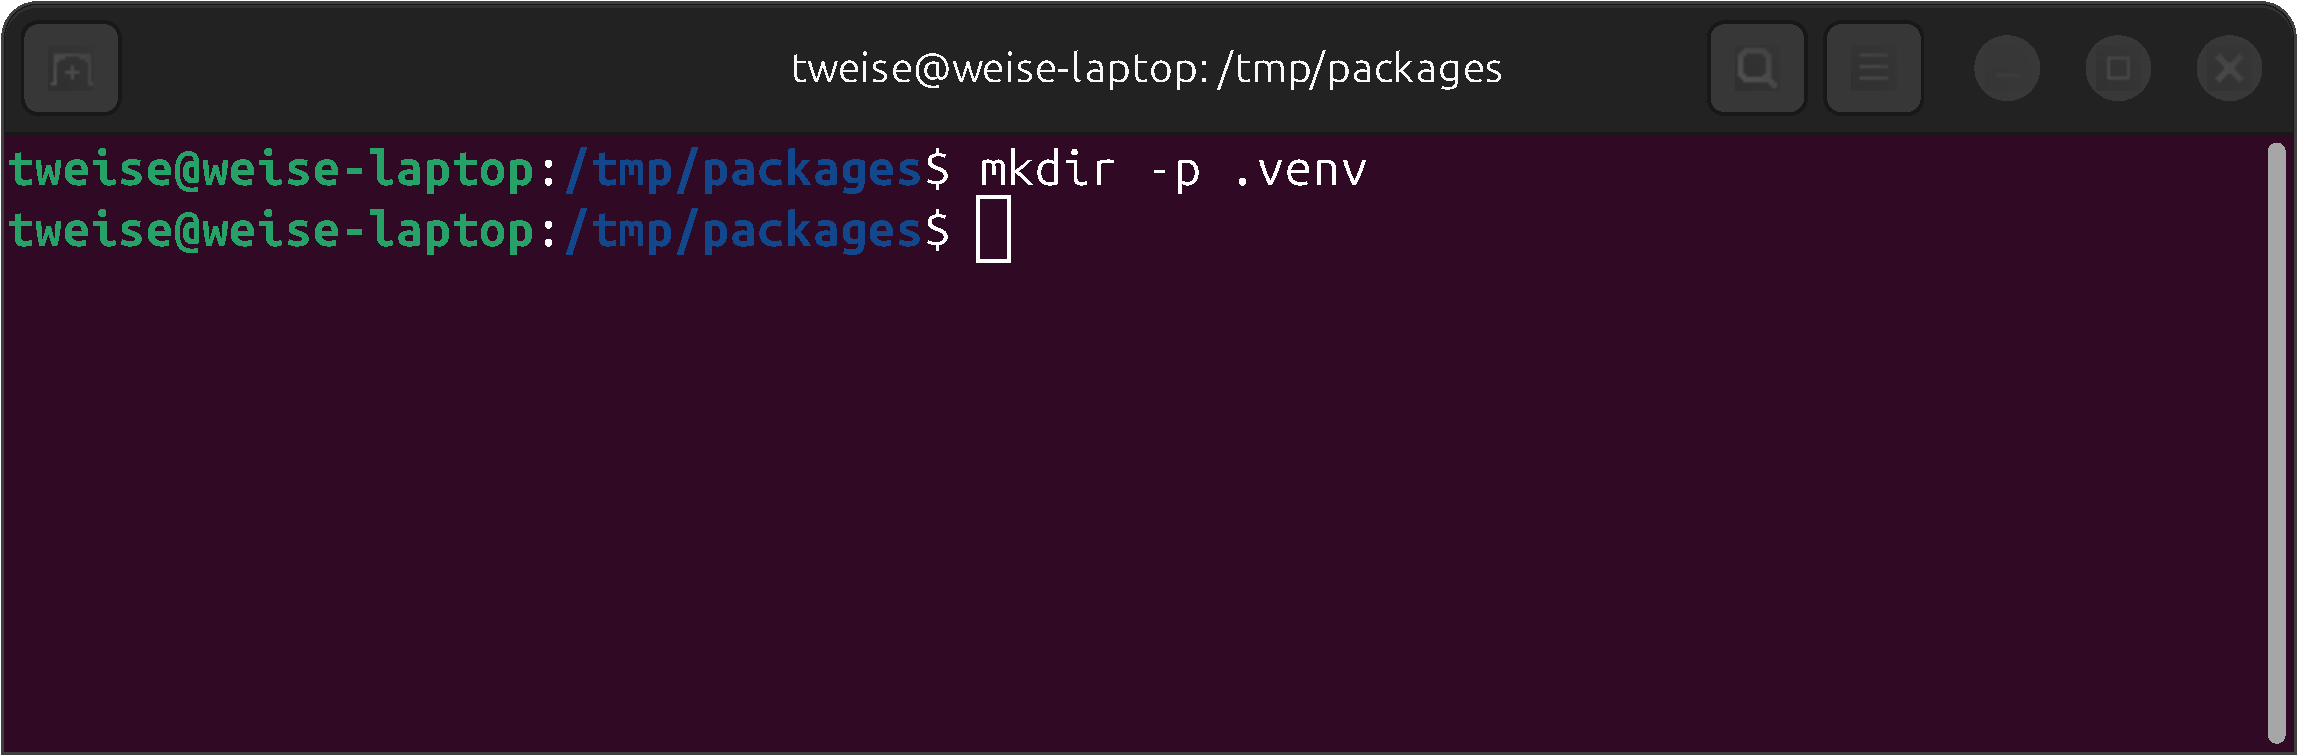
\includegraphics[width=0.48\linewidth]{\currentDir/venvLinux1}}%
%
\floatSep%
%
\subfloat[][%
Set up the \pgls{virtualEnvironment} in directory \bashil{.venv} by typing \bashil{python3 -m venv .venv} and hitting~\keys{\return}.%
\label{fig:venvLinux2}%
]{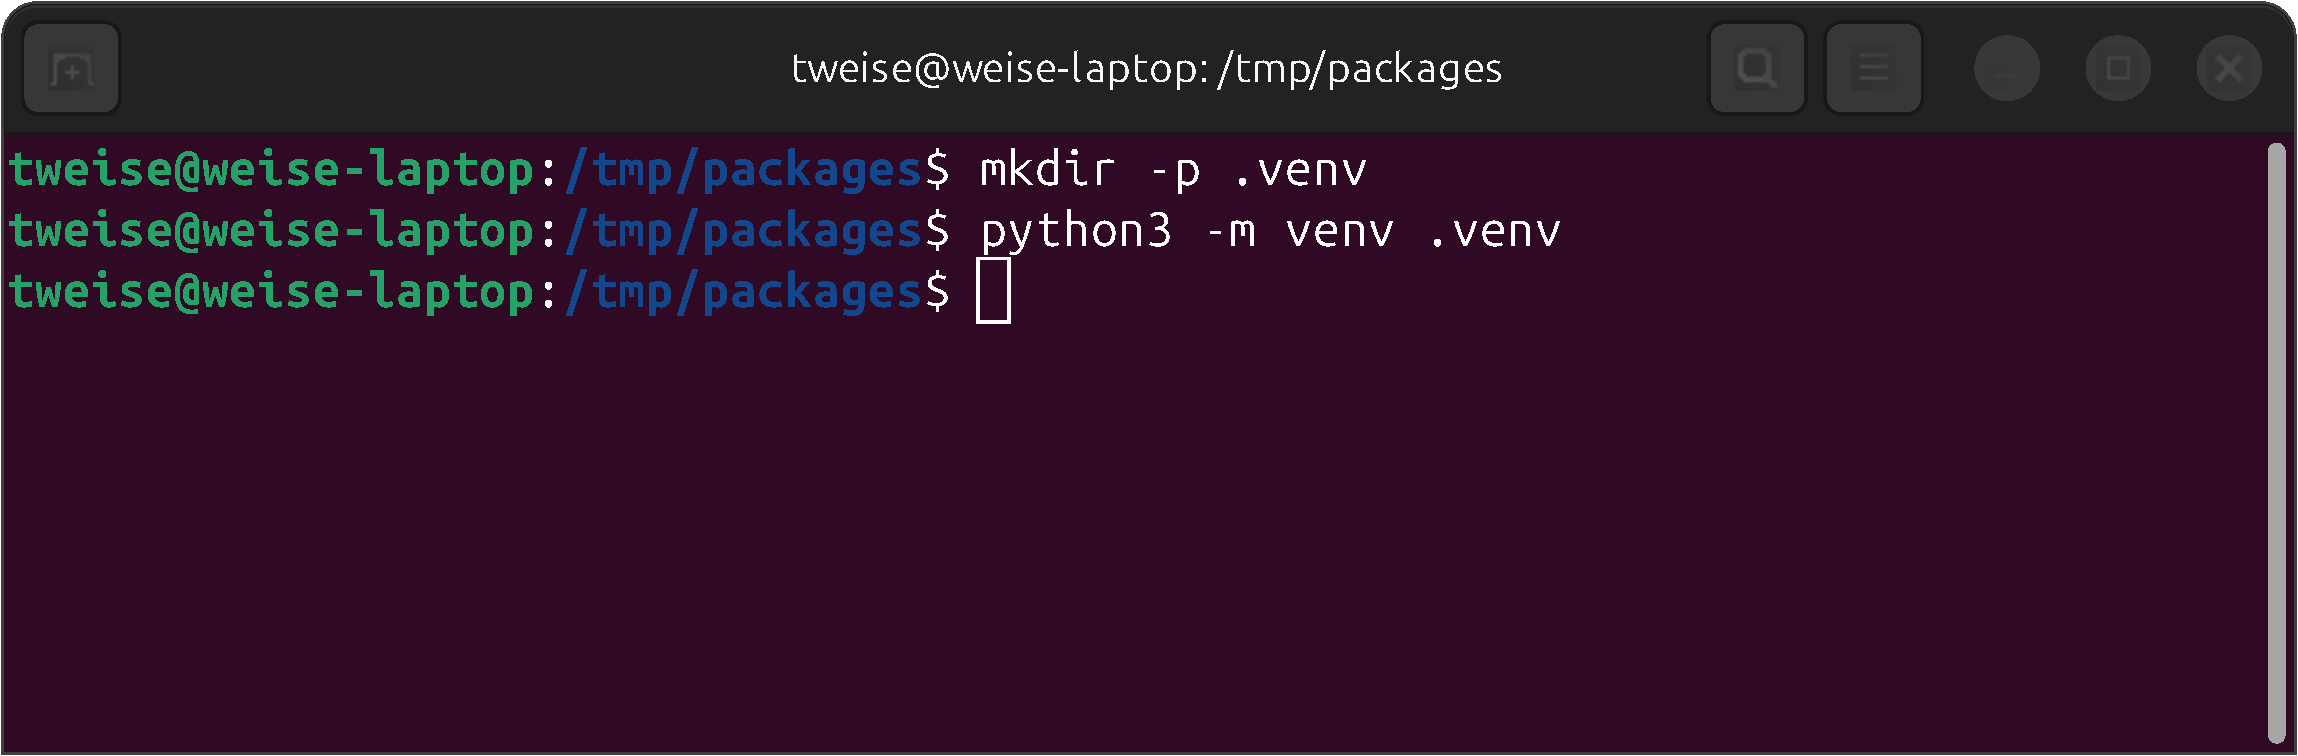
\includegraphics[width=0.48\linewidth]{\currentDir/venvLinux2}}%
%
\floatRowSep%
%
\subfloat[][%
We activate the \pgls{virtualEnvironment} by \bashil{source .venv/bin/activate} + \keys{\return}. %
Notice that the prompt changes: It now has the prefix \bashil{(.venv)}.%
\label{fig:venvLinux3}%
]{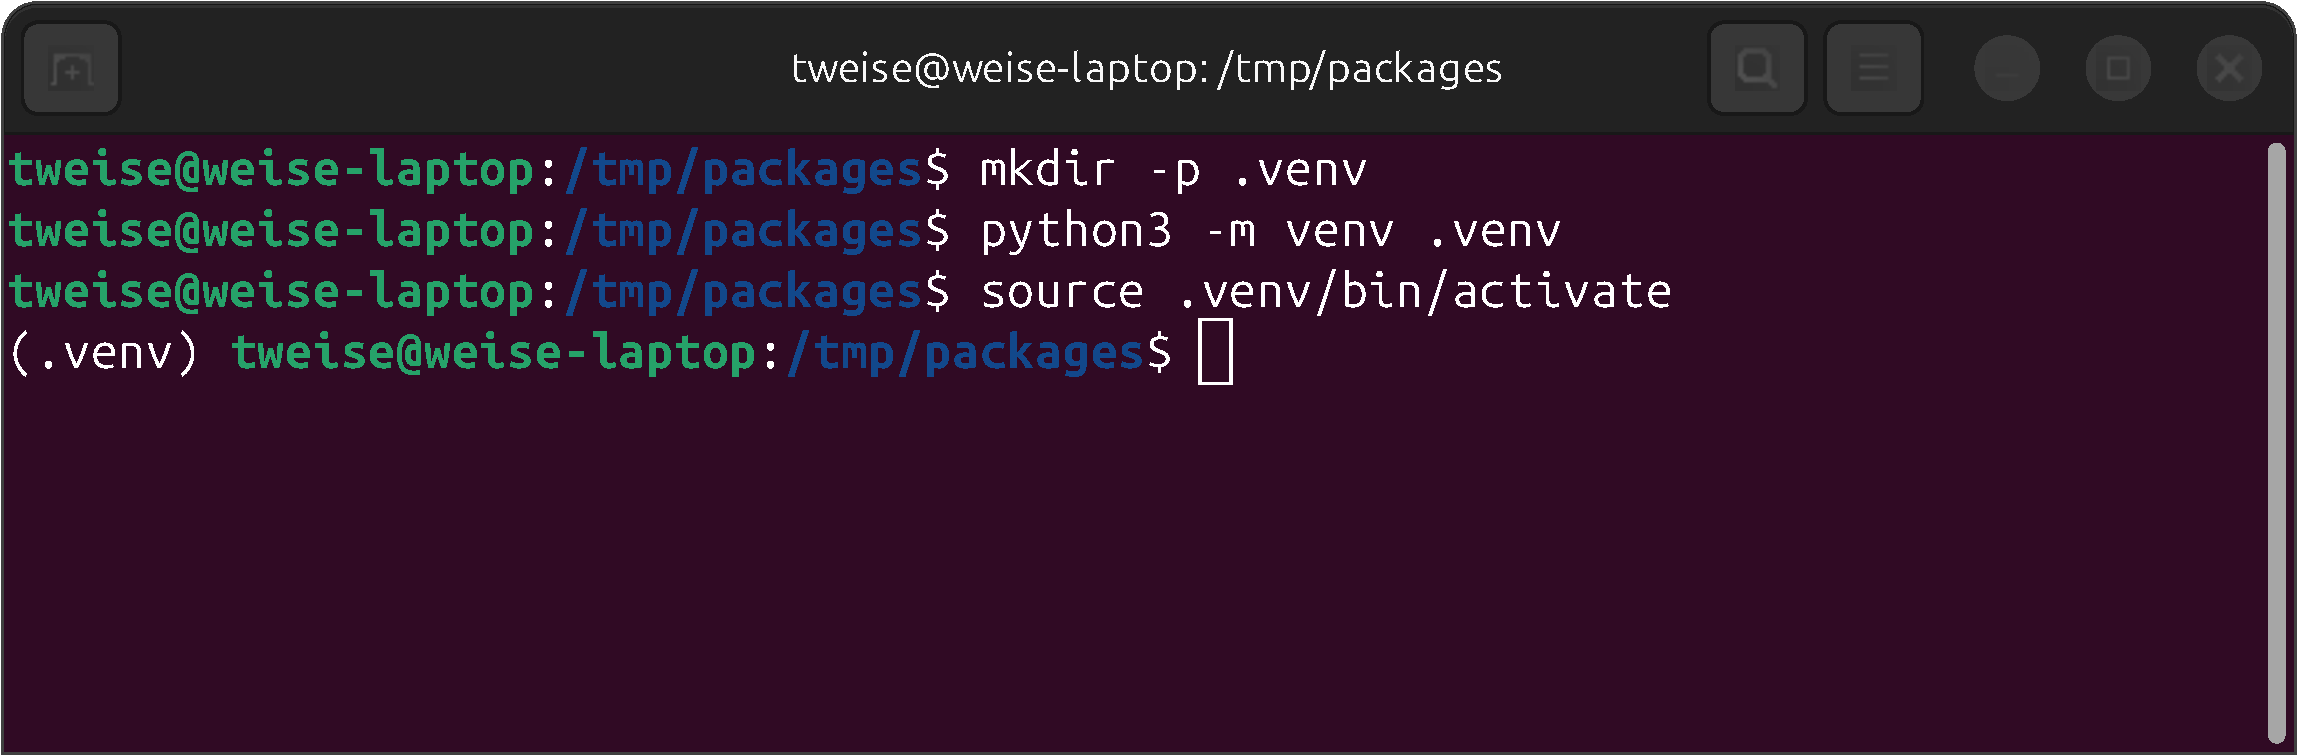
\includegraphics[width=0.48\linewidth]{\currentDir/venvLinux3}}%
%
\floatSep%
%
\subfloat[][%
We install the \numpy\pythonIdx{numpy} \pgls{package} into the activated \pgls{virtualEnvironment} vis \bashil{pip install --require-virtualenv numpy} + \keys{\return}.%
\label{fig:venvLinux4}%
]{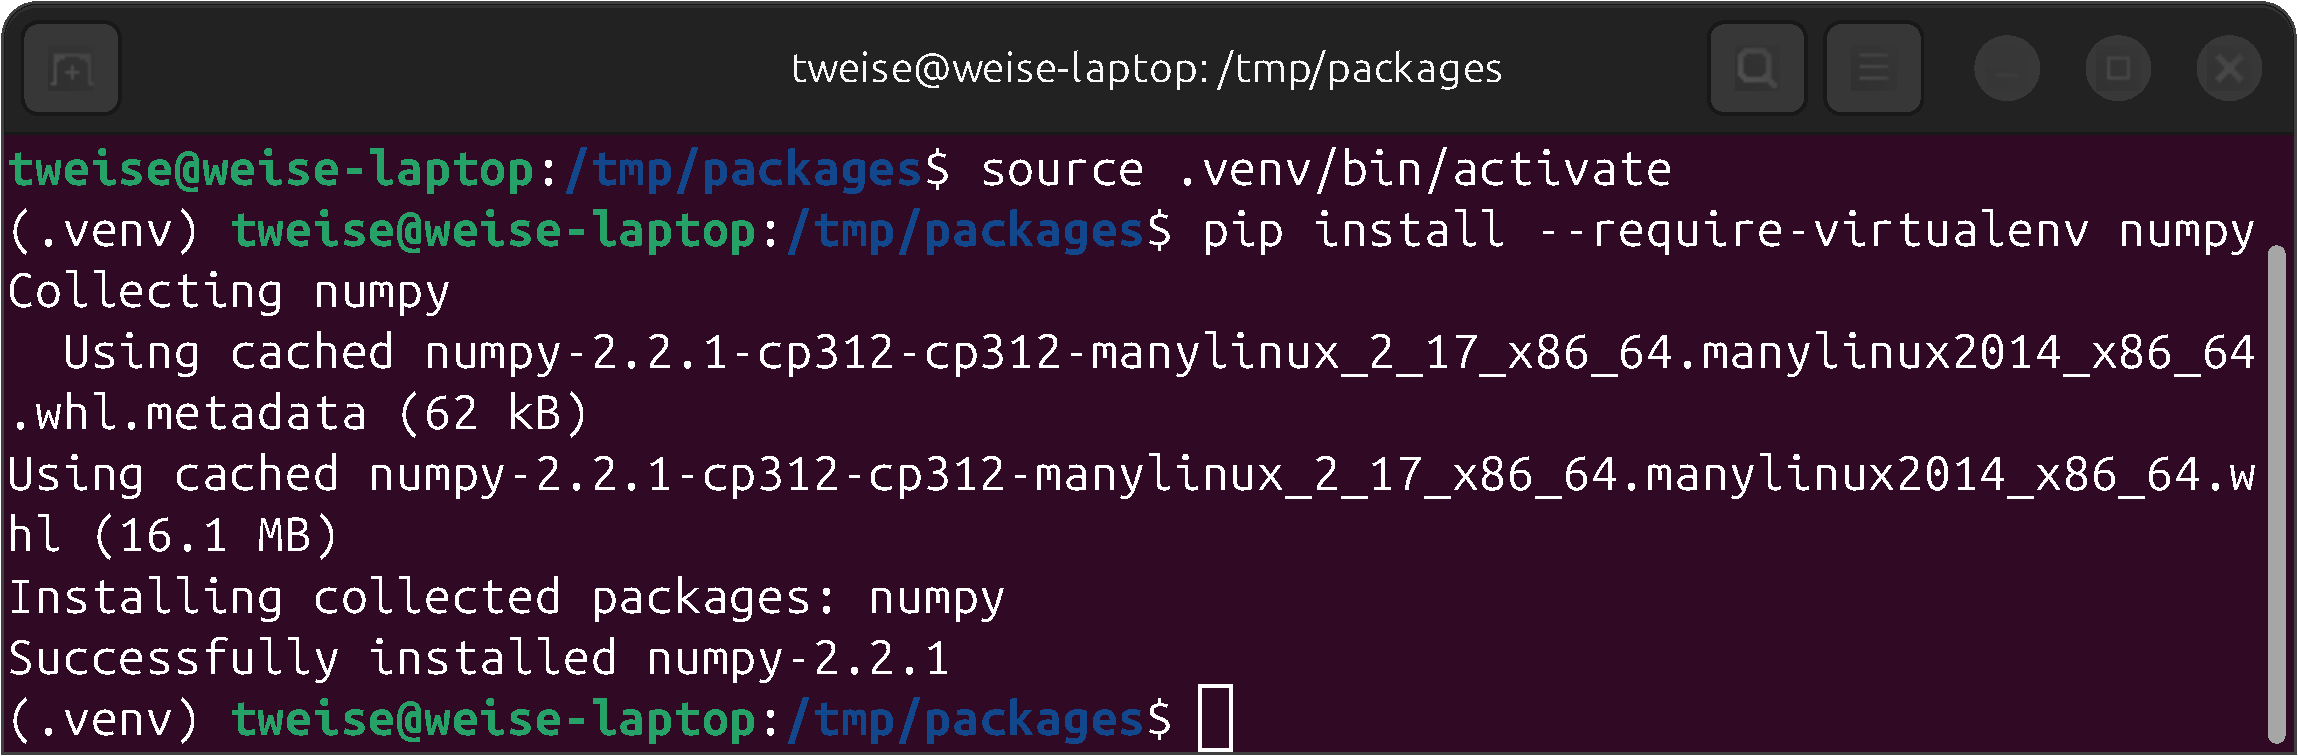
\includegraphics[width=0.48\linewidth]{\currentDir/venvLinux4}}%
%
\floatRowSep%
%
\subfloat[][%
Now we can execute the \python\ program \textil{numpy_user.py} from \cref{lst:packages:numpy_user} via \bashil{python3 numpy_user.py} + \keys{\return}.%
\label{fig:venvLinux5}%
]{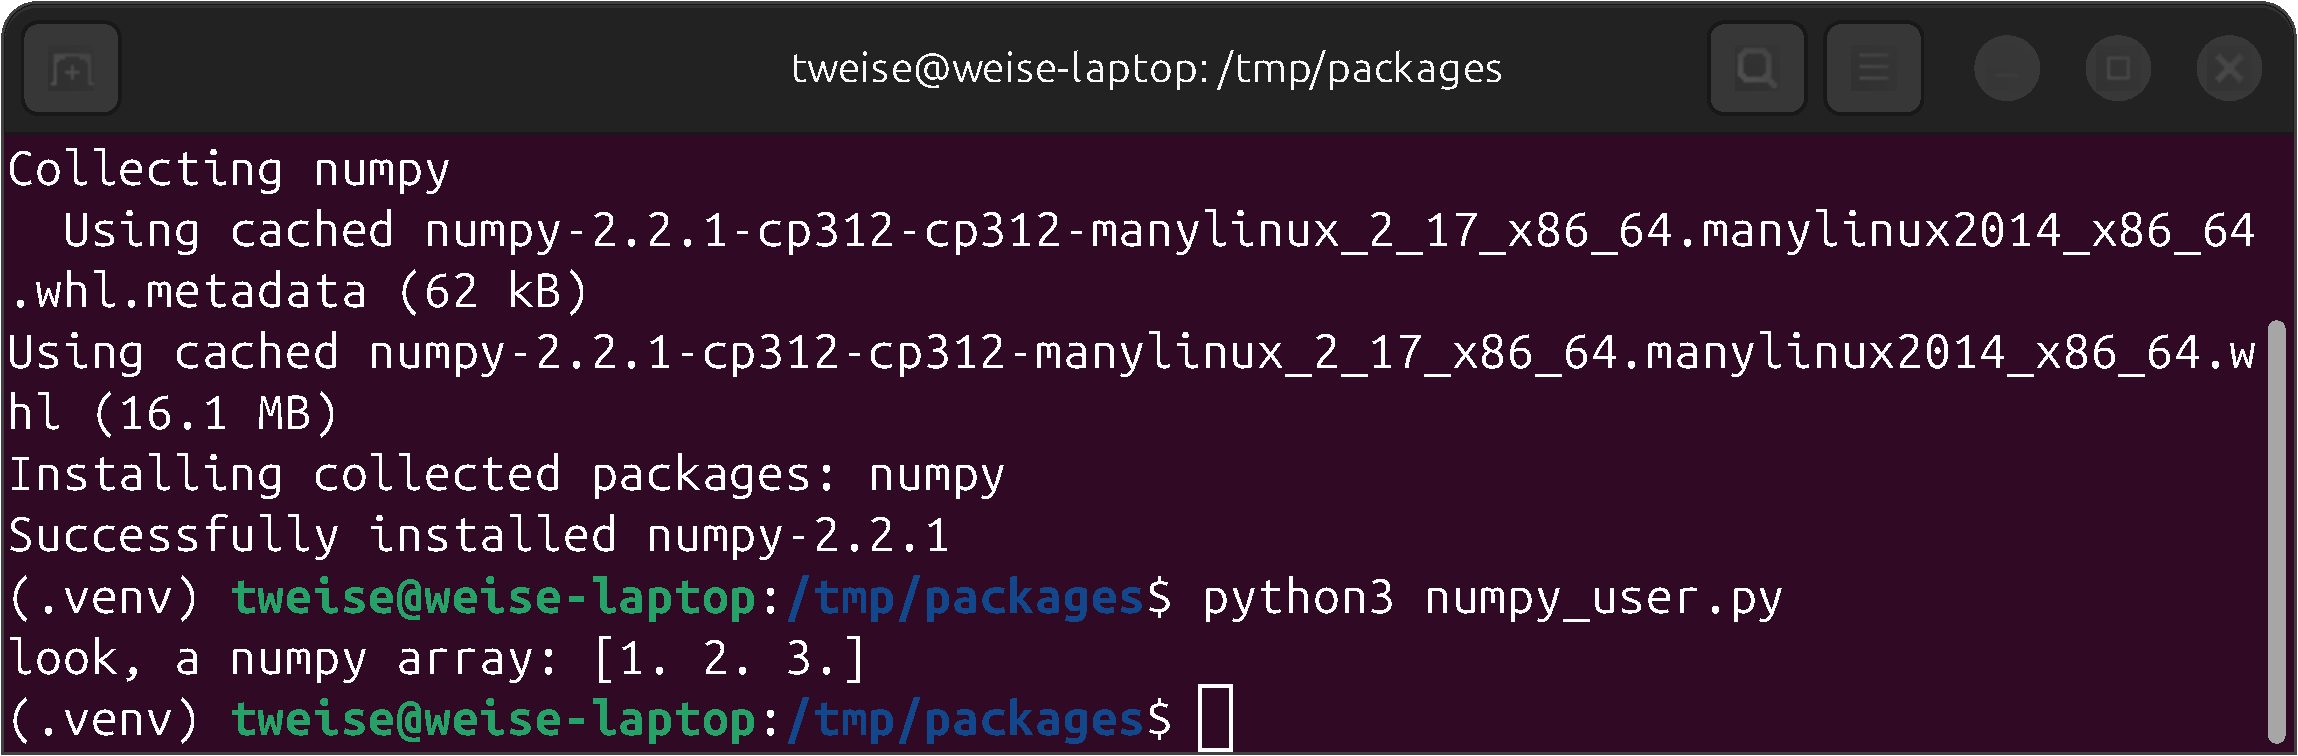
\includegraphics[width=0.48\linewidth]{\currentDir/venvLinux5}}%
%
\floatSep%
%
\subfloat[][%
We deactivate the \pgls{virtualEnvironment} by calling \bashil{deactivate} and hitting~\keys{\return}. %
We could activate it again at any point in time in the same way shown in \cref{fig:venvLinux3}.%
\label{fig:venvLinux6}%
]{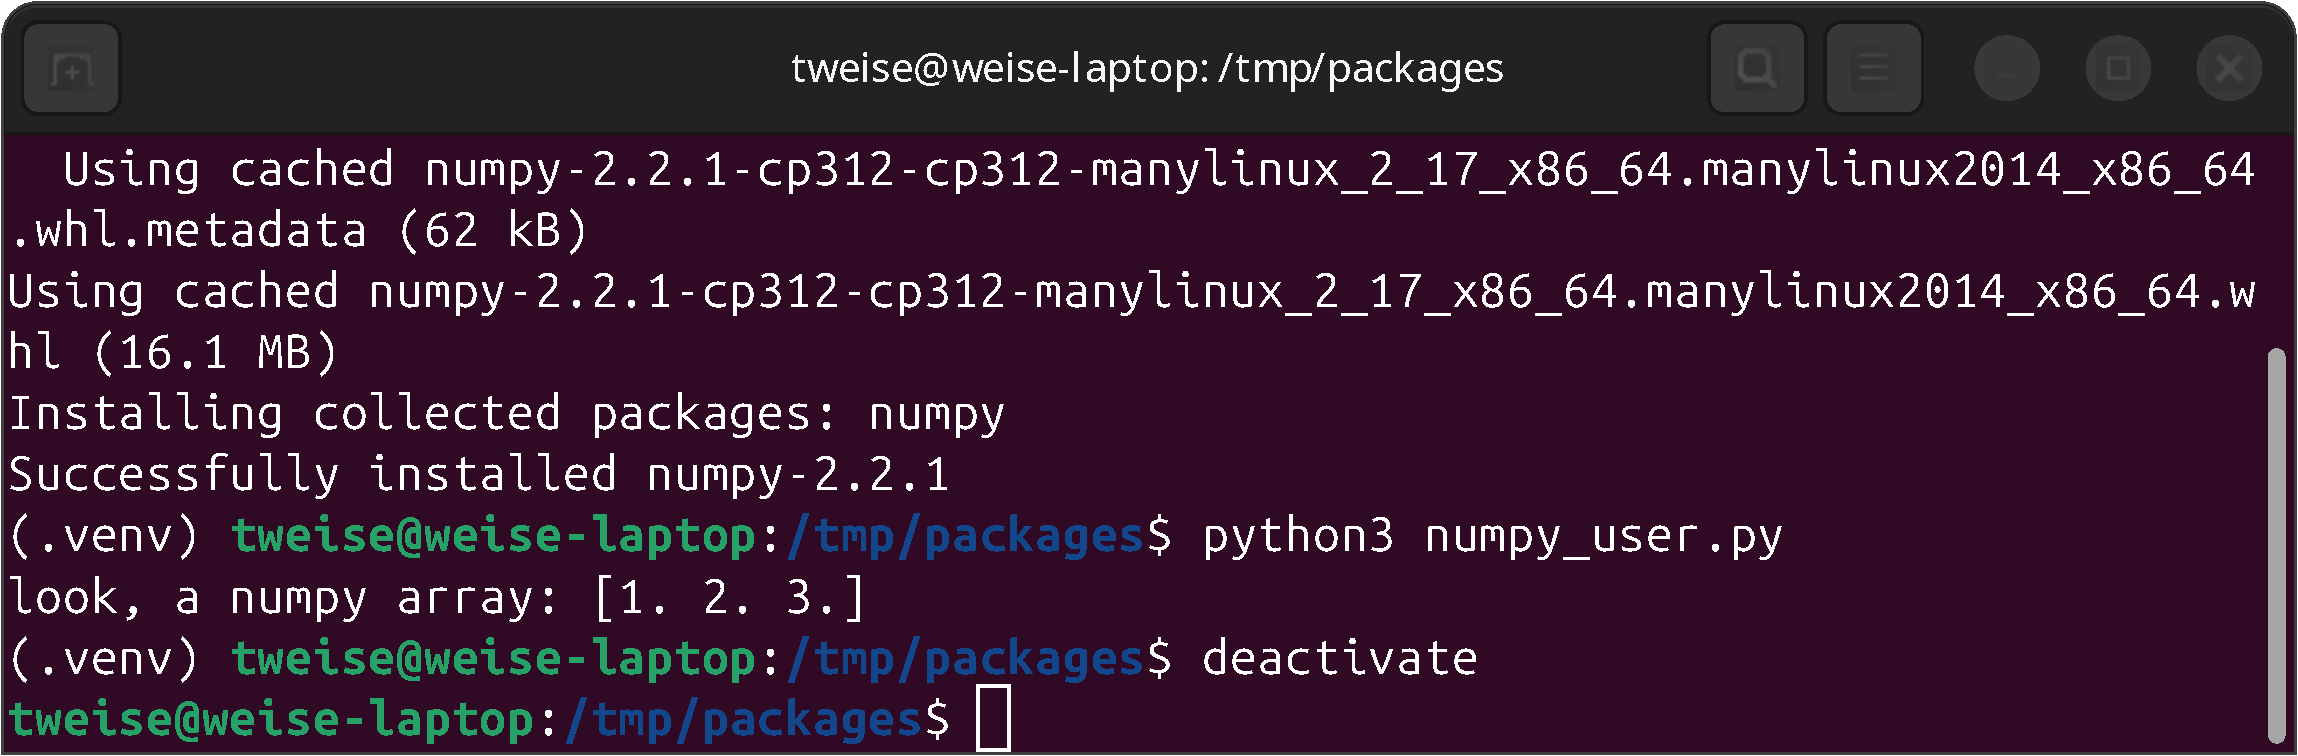
\includegraphics[width=0.48\linewidth]{\currentDir/venvLinux6}}%
%
\floatRowSep%
%
\subfloat[][%
Trying to execute \textil{numpy_user.py} will now fail, because \numpy\ is only installed in the \pgls{virtualEnvironment}, which is not active now.%
\label{fig:venvLinux7}%
]{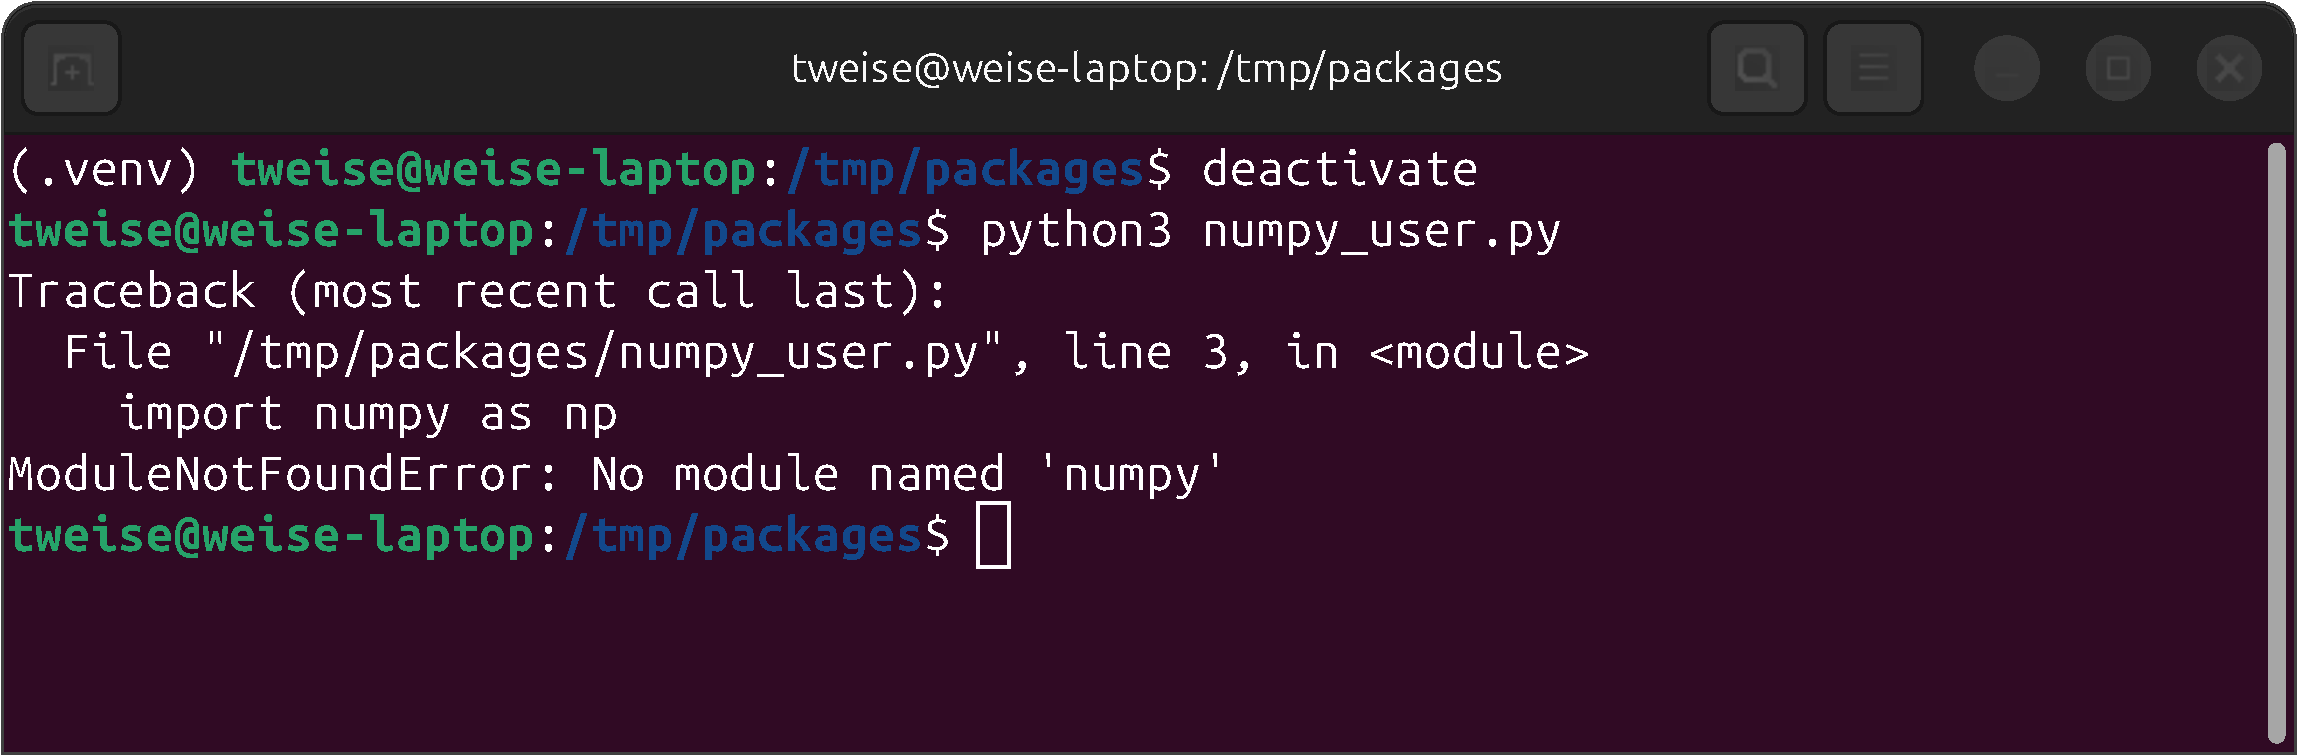
\includegraphics[width=0.48\linewidth]{\currentDir/venvLinux7}}%
%
\floatSep%
%
\subfloat[][%
Finally, we delete the directory \bashil{.venv} via \bashil{rm -rf .venv} + \keys{\return}. %
Normally, you would retain this directory and use it again next time you want to execute our program.%
\label{fig:venvLinux8}%
]{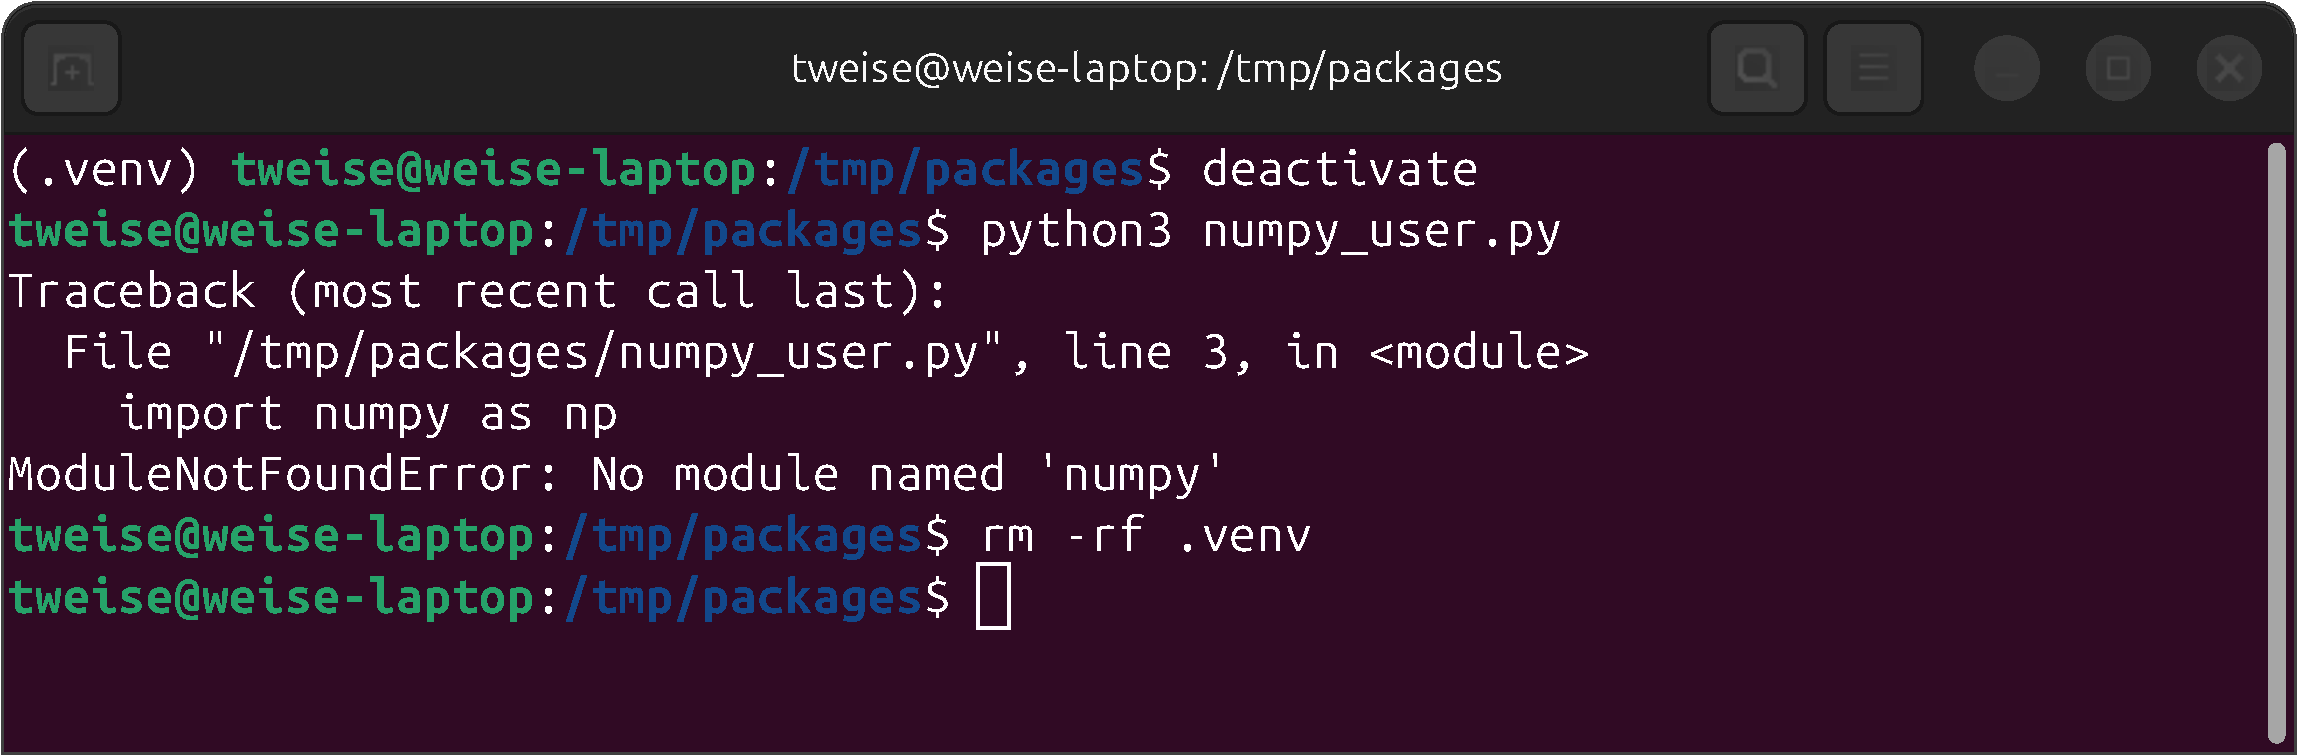
\includegraphics[width=0.48\linewidth]{\currentDir/venvLinux8}}%
%
\caption{A step-by-step execution of the commands in \cref{lst:packages:numpy_user_venv_sh} in the \ubuntu\ \linux\ \pgls{terminal}, which was opened by hitting \ubuntuTerminal.}%
\label{fig:venvLinux}%
\end{figure}%
%
\Cref{lst:packages:numpy_user_venv_sh} presents a self-contained example where we execute the necessary commands to setup a \pgls{virtualEnvironment}, install the needed package, run our program, and tear down the virtual environment.
In the real world, you would set up the environment once and could use it many times to run your program.

Assume that we have already opened a \pgls{terminal} by pressing~\ubuntuTerminal\ and that we have entered the directory where our program~\bashil{numpy_user.py} from \cref{lst:packages:numpy_user} is located.
In \cref{fig:venvLinux}, we step-by-step execute the commands from \cref{lst:packages:numpy_user_venv_sh} and show their output.
We begin by creating a new empty directory named~\bashil{.venv} in our current directory by \bashil{mkdir -p .venv} command followed by~\keys{\return}~(\cref{fig:venvLinux1}).
Inside this directory, we set up the new and empty \pgls{virtualEnvironment} by typing \bashil{python3 -m venv .venv}, again followed by~\keys{\return}~(\cref{fig:venvLinux2}).
The directory \bashil{.venv} now should contain a \python\ interpreter as well as all files needed for managing the environment.

The next step is to activate the environment.
If we would type \bashil{python3} right now, we would still be using the system's \python\ interpreter and the packages installed system-wide.
However, we actually want to use the \pgls{virtualEnvironment} instead.
For this, we need to execute \emph{all} the commands in the file \bashil{.venv/bin/activate}, which was automatically created for us when we set up the \pgls{virtualEnvironment}.
The simplest way to do this is to just copy all of them into the current \pgls{terminal} as if we had written by hand.
This happens if we type \bashil{source .venv/bin/activate}, confirmed by~\keys{\return}, as shown in \cref{fig:venvLinux3}.
If you are following this example on your own computer, then after executing this command, the \bash\ prompt (the little text on the left-hand side) changes, showing that now the \pgls{virtualEnvironment} is active.
This is also visible in \cref{fig:venvLinux3}, where the prefix~\bashil{(.venv)} is added to the prompt.

This means that any call to the \python\ interpreter will, from now on, use the interpreter stored in the \pgls{virtualEnvironment}.
We can also only use packages that were installed there.
If we execute \bashil{pip install --require-virtualenv numpy}, this will install the \numpy\ \pgls{package}.
But it uses the \python\ interpreter and \pgls{package} directory of the activated \pgls{virtualEnvironment}.
So in \cref{fig:venvLinux4}, \numpy\pythonIdx{numpy} is not installed system-wide, but into the \pgls{virtualEnvironment}.%
%
\begin{sloppypar}%
We can now execute our small program \bashil{numpy_user.py} in \cref{fig:venvLinux5}.
We type \bashil{python3 numpy_user.py} and hit~\keys{\return}.
Indeed, the expected output \textil{look, a numpy array: [1. 2. 3.]} appears in the \pgls{terminal}, as also already shown in \cref{exec:packages:numpy_user_venv_sh}.
Our program uses the local \numpy\ installation inside the \pgls{virtualEnvironment}.%
\end{sloppypar}%
%
We are now finished with our application.
To clean up, we deactivate the \pgls{virtualEnvironment} by executing~\bashil{deactivate} in \cref{fig:venvLinux6}.
This causes the prompt to change back to normal.
Any invocation of \python\ would now use the system installation.
It would no longer have access to our \pgls{virtualEnvironment} and the \pglspl{package} installed within.

If this was a more complex and useful application, then this would be the steps to get it ready and usable:
We create the \pgls{virtualEnvironment} exactly once.
Exactly once we need to install all the required \pglspl{package} into it.
Whenever we want to run our application, we would open a new \pgls{terminal}, we enter our directory, activate the \pgls{virtualEnvironment}, and then just run the program.
After that, we would deactivate the environment.
Deactivating the environment does not delete anything.
All of our settings and installed \pglspl{package} are still there.
The next time we activate the environment again, we can use them again, without the need to re-install them.

Anyway, we did deactivate the environment just now.
To confirm that we really installed \numpy\ only locally and that our program was really using the \pgls{package} installed in the \pgls{virtualEnvironment}, we try to run our program again \emph{after} deactivating the environment in \cref{fig:venvLinux7}.
As you can see in \cref{fig:venvLinux7,exec:packages:numpy_user_venv_sh}, this second execution fails:
A \pythonilIdx{ModuleNotFoundError} is raised and the interpreter terminates.%
%
\begin{sloppypar}%
Finally, in our example in \cref{lst:packages:numpy_user_venv_sh,fig:venvLinux8}, we delete the \pgls{virtualEnvironment} directory again via~\bashil{rm -rf .venv}.
Normally, you would \emph{not} do this.\footnote{%
I just clean up here because my examples are automatically executed whenever the book is built and I want to avoid that the examples interfer with each other or that, accidentally, some files from the environment land in my \git\ repositories.}
You do not want to re-create the \pgls{virtualEnvironment} again every time you execute your application.
As said, once you have installed the required \pglspl{package}, you can simply activate the environment and run your program whenever you want.%
\end{sloppypar}%
%
\FloatBarrier%
\endhsection%
%
\hsection{pip and Virtual Environments under Microsoft Windows}%
%
\begin{figure}%
\centering%
\tightbox{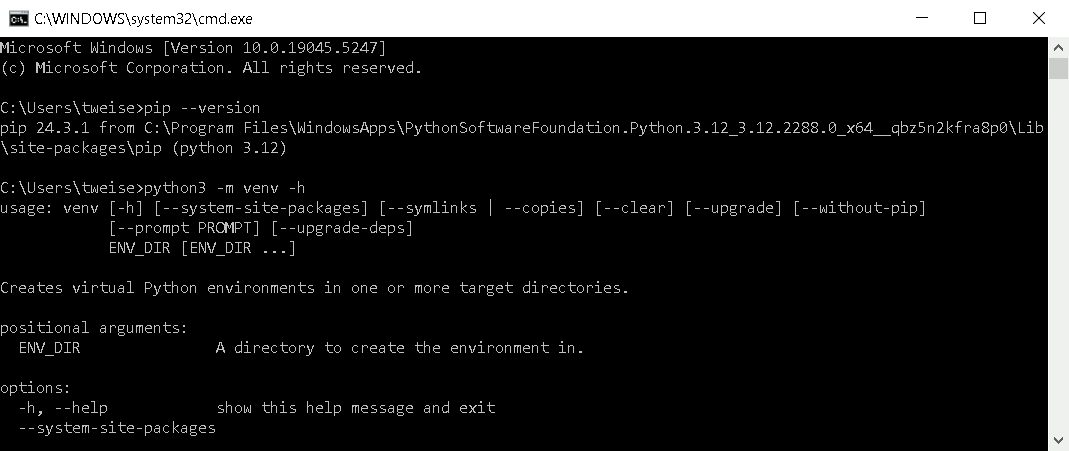
\includegraphics[width=0.85\linewidth]{\currentDir/installPipVenvWindows}}%
\caption{Installing \pip\ and \venv\ under \microsoftWindows: They are already installed.}%
\label{fig:installPipVenvWindows}%
\end{figure}%
%
Like under \linux, we also need to make sure that \pip\ and \venv\ are installed before we can actually use either of them.
Luckily, as shown in \cref{fig:installPipVenvWindows}, they already came pre-installed with my \python\ distribution.

\gitLoad{lst:packages:numpy_user_venv_bat}{\programmingWithPythonCodeRepo}{packages/numpy_user_venv.bat}{}%
\listingBash{packages:numpy_user_venv_bat}{%
An example of using \pglspl{virtualEnvironment} and \pip\ under \microsoftWindows\ to install \numpy\ and to run our program \cref{lst:packages:numpy_user}. %
The output is given in \cref{fig:venvWindowsScript,fig:venvWindows}}%
%
\begin{figure}%
\centering%
\tightbox{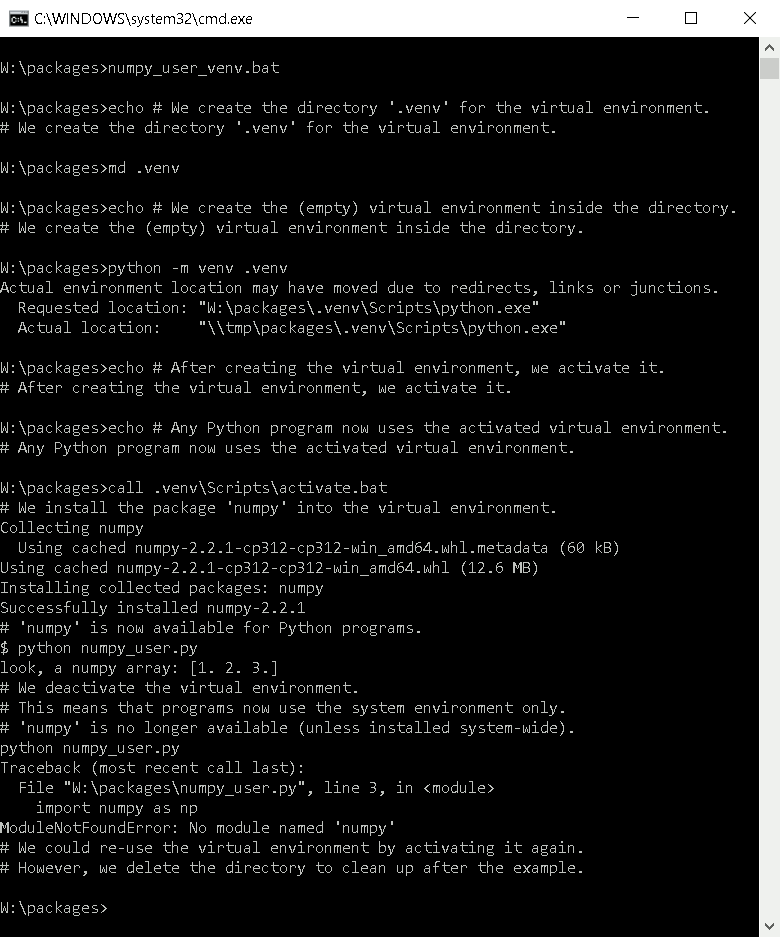
\includegraphics[width=0.75\linewidth]{\currentDir/venvWindowsScript}}%
\caption{The output of \cref{lst:packages:numpy_user_venv_bat} when executed in a \microsoftWindows\ \pgls{terminal}. %
To open the terminal, \windowsTerminal.}%
\label{fig:venvWindowsScript}%
\end{figure}%
%
\begin{figure}%
\centering%
%
\subfloat[][%
Create the directory for the \pgls{virtualEnvironment} by typing \batil{md .venv} into the \pgls{terminal} and hitting~\keys{\return}.%
\label{fig:venvWindows1}%
]{\tightbox{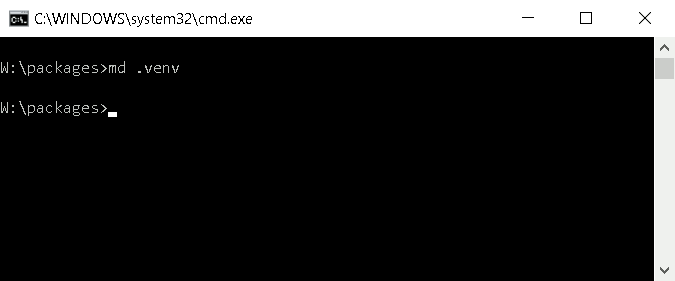
\includegraphics[width=0.48\linewidth]{\currentDir/venvWindows1}}}%
%
\floatSep%
%
\subfloat[][%
Set up the \pgls{virtualEnvironment} in directory \batil{.venv} by typing \batil{python -m venv .venv} and hitting~\keys{\return}.%
\label{fig:venvWindows2}%
]{\tightbox{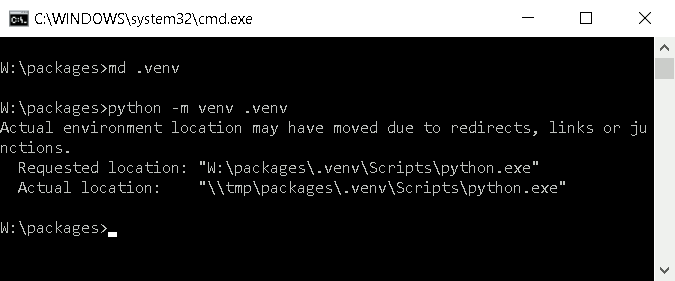
\includegraphics[width=0.48\linewidth]{\currentDir/venvWindows2}}}%
%
\floatRowSep%
%
\subfloat[][%
We activate the \pgls{virtualEnvironment} by \batil{.venv\\Scripts\\activate.bat} + \keys{\return}. %
Notice that the prompt changes: It now has the prefix~\batil{(.venv)}.%
\label{fig:venvWindows3}%
]{\tightbox{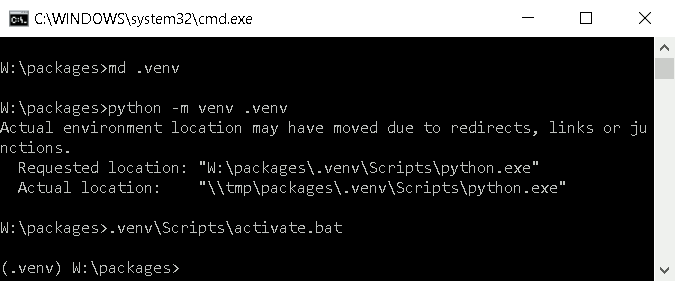
\includegraphics[width=0.48\linewidth]{\currentDir/venvWindows3}}}%
%
\floatSep%
%
\subfloat[][%
We install the \numpy\pythonIdx{numpy} \pgls{package} into the activated \pgls{virtualEnvironment} vis \batil{pip install --require-virtualenv numpy} + \keys{\return}.%
\label{fig:venvWindows4}%
]{\tightbox{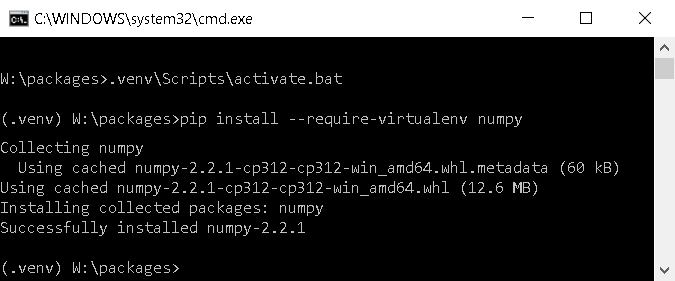
\includegraphics[width=0.48\linewidth]{\currentDir/venvWindows4}}}%
%
\floatRowSep%
%
\subfloat[][%
Now we can execute the \python\ program \textil{numpy_user.py} from \cref{lst:packages:numpy_user} via \batil{python numpy_user.py} + \keys{\return}.%
\label{fig:venvWindows5}%
]{\tightbox{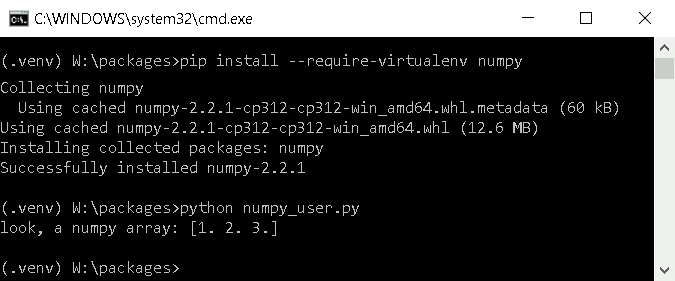
\includegraphics[width=0.48\linewidth]{\currentDir/venvWindows5}}}%
%
\floatSep%
%
\subfloat[][%
We deactivate the \pgls{virtualEnvironment} by calling \batil{deactivate} and hitting~\keys{\return}. %
We could activate it again at any point in time in the same way shown in \cref{fig:venvWindows3}.%
\label{fig:venvWindows6}%
]{\tightbox{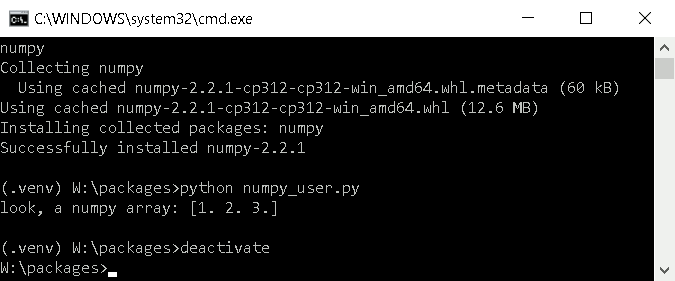
\includegraphics[width=0.48\linewidth]{\currentDir/venvWindows6}}}%
%
\floatRowSep%
%
\subfloat[][%
Trying to execute \textil{numpy_user.py} will now fail, because \numpy\ is only installed in the \pgls{virtualEnvironment}, which is not active now.%
\label{fig:venvWindows7}%
]{\tightbox{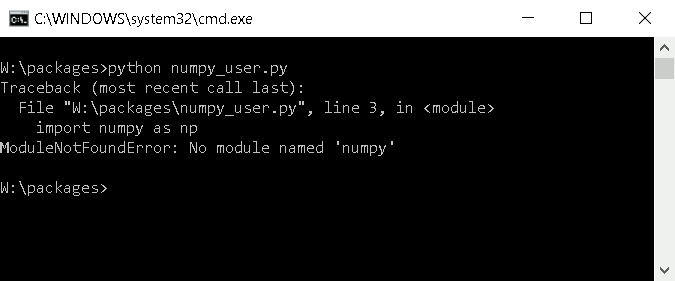
\includegraphics[width=0.48\linewidth]{\currentDir/venvWindows7}}}%
%
\floatSep%
%
\subfloat[][%
Finally, we delete the directory \batil{.venv} via \batil{rd /S /Q .venv} + \keys{\return}. %
Normally, you would retain this directory and use it again next time you want to execute our program.%
\label{fig:venvWindows8}%
]{\tightbox{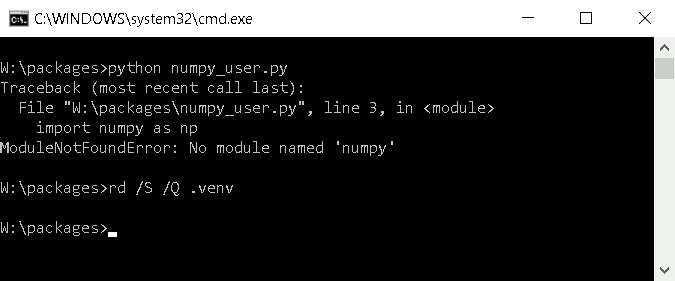
\includegraphics[width=0.48\linewidth]{\currentDir/venvWindows8}}}%
%
\caption{A step-by-step execution of the commands in \cref{lst:packages:numpy_user_venv_bat} in the \microsoftWindows\ \pgls{terminal}. %
To open the terminal, \windowsTerminal.}%
\label{fig:venvWindows}%
\end{figure}%

We now want to execute our small program \cref{lst:packages:numpy_user}, which uses \numpy.
\numpy\pythonIdx{numpy} does not come pre-installed.
So we need to install it first.
Following general best practices, we will do so using a virtual environment.
All the necessary commands for this are listed in the \microsoftWindows\ batch file in \cref{lst:packages:numpy_user_venv_bat}.
The complete corresponding output in the \pgls{terminal} is given in \cref{fig:venvWindowsScript}.

Here, we will work our way through this step-by-step in \cref{fig:venvWindows}.
First, you need to \windowsTerminal\ to open a \microsoftWindows\ \pgls{terminal}.
We enter the directory where our program file \batil{numpy_user.py} is located with the \batil{cd}~commend~(not illustrated).

As a first step, we need to create a directory \batil{.venv} to host the \pgls{virtualEnvironment}.
We therefore write \batil{md .venv} and hit~\keys{\return} in~\cref{fig:venvWindows1}.
To then set up a new and, initially, empty \pgls{virtualEnvironment} in this directory, we type \batil{python -m venv .venv} and hit~\keys{\return}~(see \cref{fig:venvWindows2}).
Notice that under \ubuntu\ \linux, we always used the \bashil{python3} command, but here we always use \batil{python} instead.
Either way, executing the command has filled the directory \batil{.venv} with the necessary files and scripts for an isolated \python\ environment.

In \cref{fig:venvWindows3}, we activate this environment by running \batil{.venv\\Scripts\\activate.bat} (and hitting~\keys{\return}).
This \microsoftWindows\ batch file has been created for us when we set up the \pgls{virtualEnvironment}.
It activates the environment, which leads to a change in the prompt, i.e., the little text that always appears left of where we type the input.
As can be seen in \cref{fig:venvWindows3}, the text \batil{(.venv)} has been pre-pended to the prompt, which tells us that this is the currently active \pgls{virtualEnvironment}.

We now want to install the \numpy\pythonIdx{numpy} \pgls{package} into this \pgls{virtualEnvironment}.
We can do this by typing \batil{pip install --require-virtualenv numpy} and then pressing~\keys{\return}.
This causes \numpy\ to be downloaded (or copied from the internal cache) and installed, as shown in \cref{fig:venvWindows4}.%
%
\begin{sloppypar}%
We can now run our program \textil{numpy_user.py} by typing \batil{python numpy_user.py} and hitting~\keys{\return}.
Indeed, as you can see in \cref{fig:venvWindows5}, the program runs without error and prints \textil{look, a numpy array: [1. 2. 3.]}, exactly as expected.
It found the \numpy\pythonIdx{numpy} \pgls{package} that was installed in the \pgls{virtualEnvironment}.%
\end{sloppypar}%
%
Now that we have finished executing our program, we can deactivate the \pgls{virtualEnvironment}.
In \cref{fig:venvWindows6}, we type \batil{deactivate} and press~\keys{\return}.
This causes the prompt to change back to normal.
The \pgls{virtualEnvironment} is no longer active.
This means that from now on, all interaction takes place with the system \python\ installation.
If our program was a real, valuable application, then the next time we would like to use it, we would simply activate the \pgls{virtualEnvironment} again.
All of our files, settings, and installed \pglspl{package} are still there.
Nothing has been deleted~(yet).
If we would activate the \pgls{virtualEnvironment} again, we could just run the program again, we would not need to re-installed any package.

However, we now want to verify that deactivating the \pgls{virtualEnvironment} really means that right now, we are just working with the system \python\ setup.
For this purpose, we try to run our program again \cref{fig:venvWindows7} by again writing \batil{python numpy_user.py} and hitting~\keys{\return}.
As you can see, this does not work.
\numpy\ was only installed in the \pgls{virtualEnvironment} and is not available system-wide.
The first line of our program, which tries to \pythonil{import numpy}, therefore raises a~\pythonilIdx{ModuleNotFoundError}.

At the very end of this example, I want to clean up my folder by typing \batil{rd /S /Q .venv} and hitting~\keys{\return}.
This deletes the directory \batil{.venv} and everything within.
You would normally not do this, because normally we want to re-use our \pglspl{virtualEnvironment} by activating and deactivating them as needed.
Either way, this was a complete example for using \pglspl{virtualEnvironment}, \pip, and \venv\ under \microsoftWindows.
It was actually not very much different from the \ubuntu\ \linux\ example in the previous section.%
%
\endhsection%
%
\FloatBarrier
%
\endhsection%
%
